\documentclass[12pt,letterpaper]{article}

\usepackage[protrusion=true,expansion=true]{microtype}  % Better typography
\usepackage{mathpazo}
\usepackage[T1]{fontenc}
\usepackage{setspace}
\usepackage[margin=1in]{geometry}
\usepackage{enumitem}
\usepackage{titlesec}
\usepackage[breaklinks]{hyperref}
\usepackage{tikz}
	\usetikzlibrary{positioning}
\usepackage{sidecap}
\usepackage{graphicx}

% For code samples
\usepackage{textcomp}
\usepackage{listings}
\usepackage{color}


% Import settings, which are stored in a separate file for convenience
% Syntax highlighting colors
\definecolor{lightgray}{rgb}{0.9, 0.9, 0.9}
\definecolor{darkgray}{rgb}{0.4, 0.4, 0.4}
\definecolor{purple}{rgb}{0.65, 0.12, 0.82}

\lstdefinelanguage{JavaScript}{
	keywords={break, case, catch, continue, debugger, default, delete, do, else, false, finally, for, function, if, in, instanceof, new, null, return, switch, this, throw, true, try, typeof, var, void, while, with},
	morecomment=[l]{//},
	morecomment=[s]{/*}{*/},
	morestring=[b]',
	morestring=[b]",
	ndkeywords={class, export, boolean, throw, implements, import, this},
	sensitive=true
}

\lstdefinestyle{js}{
	language=JavaScript,
	keywordstyle=\color{blue}\bfseries,
	ndkeywordstyle=\color{darkgray}\bfseries,
	identifierstyle=\color{black},
	commentstyle=\color{purple}\ttfamily,
	stringstyle=\color{red}\ttfamily,
	tabsize=2
}

\lstdefinestyle{html}{
	language=HTML,
	keywordstyle=\color{blue}\bfseries,
	ndkeywordstyle=\color{darkgray}\bfseries,
	identifierstyle=\color{black},
	commentstyle=\color{purple}\ttfamily,
	stringstyle=\color{red}\ttfamily,
	tabsize=4
}


% Set global defaults for code listings
\lstset{
	backgroundcolor=\color{lightgray},
	basicstyle=\singlespacing\footnotesize\ttfamily,
	breaklines=true,
	captionpos=b,
	extendedchars=true,
	showspaces=false,
	showstringspaces=false,
	showtabs=false,
	upquote=true
}


% Sensible defaults for spacing and line breaks
\def\UrlBreaks{\do-\do_}
\titlespacing*{\section}{0pt}{0pt}{0pt}
\titlespacing*{\subsection}{0pt}{0pt}{0pt}
\doublespacing
\makeatletter


% Customize title
\renewcommand{\maketitle}{
	\begin{flushright}
		\@author\\\@date
	\end{flushright}
	\begin{center}
		{\LARGE\@title}
	\end{center}
}


% Set title
\title{\textbf{Angular vs. React}}
\author{William Gaul\\{ICS 419: Prof. Streveler}}
\date{\today}


\begin{document}
\maketitle

\renewcommand{\abstractname}{Executive Summary}
\begin{singlespace*}
\begin{abstract}
	The modern web is inherently dynamic. As the Internet has evolved -- as JavaScript plays an increasingly ubiquitous role and applications grow in size and complexity -- developers have turned ever more toward web frameworks to make sense of the chaos. Many companies now favor applicants who have experience working with these frameworks, and so a good understanding of their usage and purpose is crucial. Why do they exist? What problems do they purport to solve, if any? How will they benefit developers and end users alike? This project aims to answer these questions by examining two very popular web frameworks in more detail: Angular and React.
\end{abstract}
\end{singlespace*}

\section{The Web, Then and Now}

\cite{Schlensker:2014}
\cite{Angular:Docs}
\cite{Hunt:2013}
\cite{Green:2013}
\cite{Hunt:2014}

\includegraphics[width=0.9\textwidth]{hello-world.png}

%This project aims to answer these questions by examining two very popular web frameworks in more detail: Angular and React. These frameworks were chosen in part for their popularity, but they also happen to take contrasting approaches to managing and abstracting application development. On the one hand, Angular offers an expressive extension of HTML specifically designed for dynamic views, centered on a concept called “two-way data binding.” On the other hand, React uses a component system that makes it easy to reason about application architecture, powered by “one-way data binding.”
%By evaluating both frameworks against a common baseline (tentatively, a simple example of DOM manipulation via a dropdown and input field), it is possible to gain a cursory understanding of their designs – that is, how they work and what they intend to do. More information can be gleaned from extensive documentation and numerous tutorials online; in particular, the Angular and React websites will reveal a great deal about goals and objectives. Although the purpose of this project is not to decide which framework is “better,” an appraisal of both frameworks on qualities such as “intuitive” and “testable” will be conducted, as it can be a helpful reflection of good application design in general.
%It is hoped that this project will inspire any budding web developers in the class to embrace web frameworks and the design principles that they afford. Moreover, as graduation approaches, studying this subject should be good preparation for entering the web development industry.



%~15 pages

%1. A well-chosen TITLE
%2. A brief Executive Summary (Abstract) of the Project
%3. A literature review of this topic (as appropriate)
%4. A written discussion of your project
%5. A discussion of any ethical issues you encountered while researching or preparing your project
%6. A well-annotated bibliography of the references and materials you used in the course of preparing your project
%7. A conclusion – What did you learn from all this?






% \cite[p.~4]{Poole:2010}. Figure \ref{fig:AESystem} shows a visualization of the relationship between the agent and its environment.

\begin{SCfigure}[][h]
	\centering
	\caption{A very simplified view of an isolated agent-environment system. The agent impacts the environment through its actions, and is influenced by its perception of the environment.}
	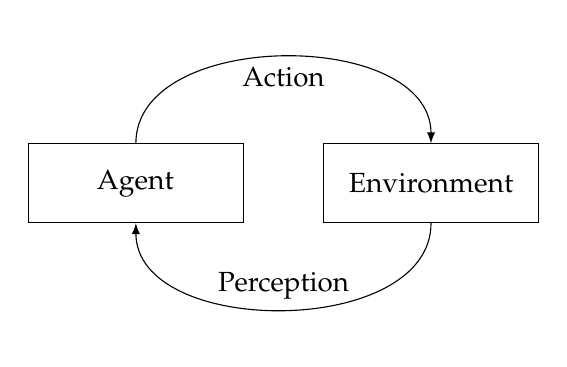
\begin{tikzpicture}[
		node distance=1.5cm and 1cm,
		ar/.style={->, >=latex},
		mynode/.style={draw, text width=2.5cm, minimum height=1cm, align=center}
	]
		\node[mynode] (agent) {Agent};
		\node[mynode,right=of agent] (env) {Environment};
		\draw[ar] (agent.north) to[out=90,in=90] node[below] {Action} (env.north);
		\draw[ar] (env.south) to[out=-90,in=-90] node[above] {Perception} (agent.south);
	\end{tikzpicture}
	\label{fig:AESystem}
\end{SCfigure}

%\footnote{}

%\begin{quote}
%	\singlespacing
%	For each possible percept sequence, a rational agent should select an action that is expected to maximize its performance measure, given the evidence provided by the percept sequence and whatever built-in knowledge the agent has.
%\end{quote}


\newpage

\appendix
\section{Code Listings}

\subsection*{Pure JavaScript}

\lstinputlisting[style=html,caption={index.html},label={lst:pureHTML}]{../examples/pure-js/index.html}
\lstinputlisting[style=js,caption={app.js},label={lst:pureJS}]{../examples/pure-js/app.js}

\newpage

\subsection*{Angular}

\lstinputlisting[style=html,caption={index.html},label={lst:angularHTML}]{../examples/angular/index.html}
\lstinputlisting[style=js,caption={app.js},label={lst:angularJS}]{../examples/angular/app.js}

\newpage

\subsection*{React}

\lstinputlisting[style=html,caption={index.html},label={lst:reactHTML}]{../examples/react/index.html}
\lstinputlisting[style=js,caption={app.js},label={lst:reactJS}]{../examples/react/app.js}

\newpage

% BIBLIOGRAPHY (Note: We use a special version of IEEEtran that has sorting and annotations)
\begin{flushleft}
\begin{singlespace*}
	\bibliographystyle{./IEEEtran}
	\bibliography{angular-vs-react}
\end{singlespace*}
\end{flushleft}

\end{document}
